% !TeX root = ../main.tex

\chapter{系统概要设计}

\section{系统概述}
本系统是针对RISC-V芯片开发团队在系统软件开发和移植过程中使用的体系结构模拟器.将编译好的RISC-V架构可执行代码加载到模拟器上运行,观察执行结果,能够脱离实际硬件平台进行系统软件的调试,也能帮助开发人员及时发现硬件实现可能存在的缺陷,从而提高整个芯片开发过程的效率。

\section{系统静态结构}
RISC-V指令集模拟器的整体功能模块如图\ref{fig:sim_general}所示,主要包含四个功能模块:预加载模块,指令流执行模块,调试模块和UI显示模块。其中,预加载模块包括模拟器参数配置,指令集注册,加载elf文件功能;指令流执行模块包括了主要的Hart模拟,中断控制器模拟,内存模拟,外设模拟等功能,是模拟器的主体功能模块;调试模块包括断点设置,内存查询,模拟中断信号发送功能;UI显示模块包括目标层序执行窗口,调试窗口等的可视化界面和模拟器状态查询功能。
\begin{figure}[H]
  \centering
  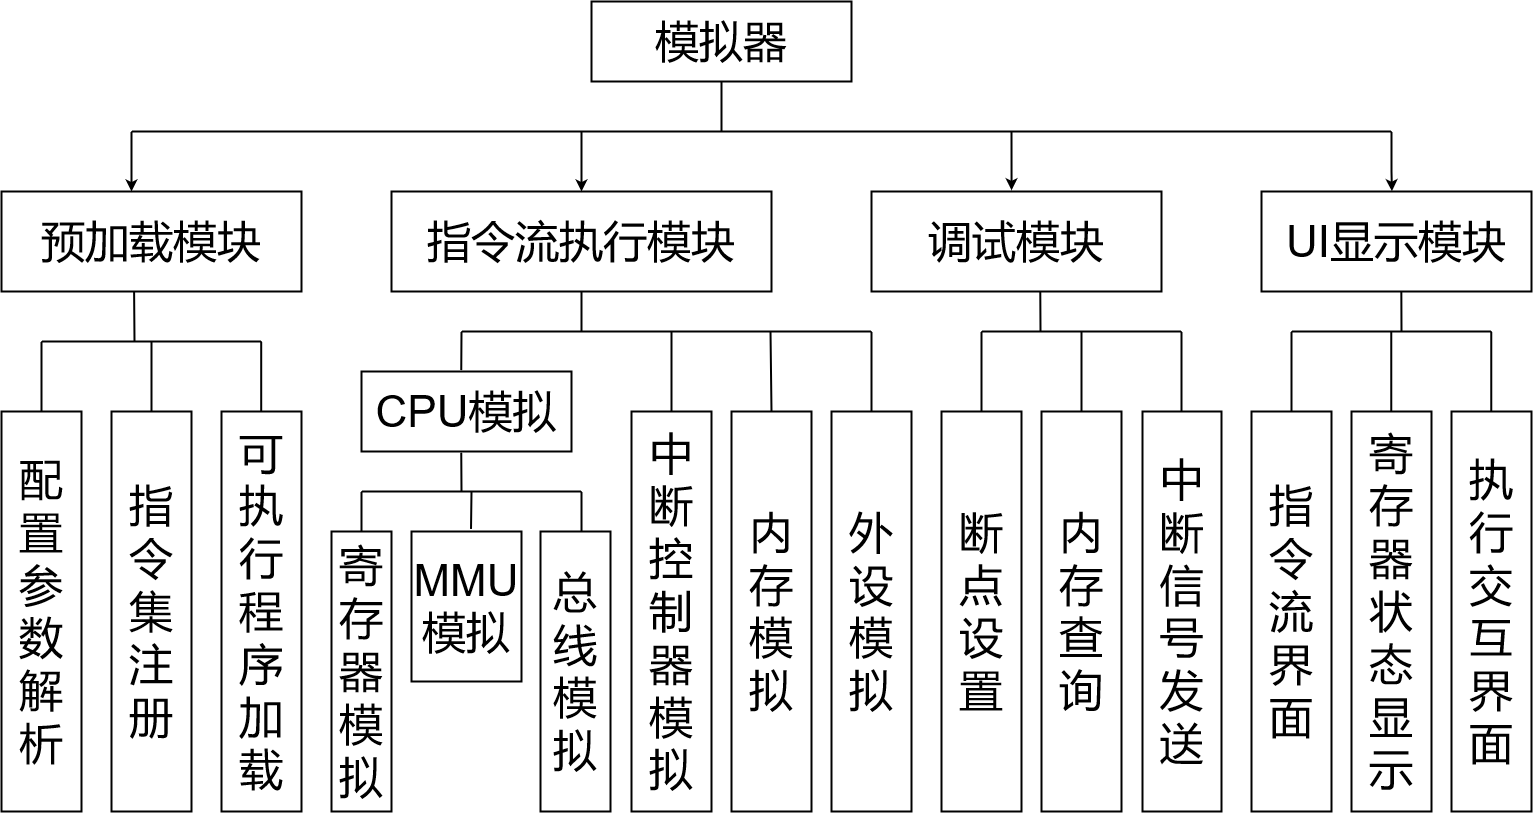
\includegraphics[width=1.0\textwidth]{sim-general.png}
  \caption{模拟器整体功能模块图}
  \label{fig:sim_general}
\end{figure}


指令流执行模块是模拟器的主体功能模块,该模块模拟了单条指令执行过程的硬件行为,包括寄存器,总线,内存,MMU,缓存,通过内存映射的I/O设备等。模拟出的RISC-V CPU整体架构如图\ref{fig:cpu}所示,每个处理器都有独立的寄存器组,内存管理单元,所有处理器共享同一个iCache,dCache,紧随其后的是L2Cache和主存。
\begin{figure}[H]
  \centering
  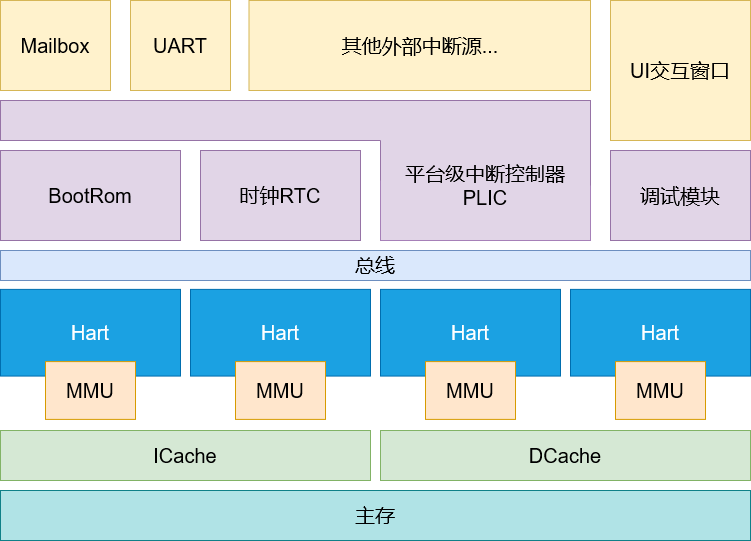
\includegraphics[width=0.8\textwidth]{cpu.png}
  \caption{处理器结构图}
  \label{fig:cpu}
\end{figure}


处理器通过总线和其他内存映射的I/O设备通信,包括BootRom,RTC,UART串口控制器,平台级中断控制器,Mailbox等等.

\section{系统动态结构}
本模拟器是trace-accurate的指令集模拟器(功能模拟器),模拟器运行的基本流程如图~\ref{fig:sim-seq}所示。
\begin{figure}[H]
  \centering
  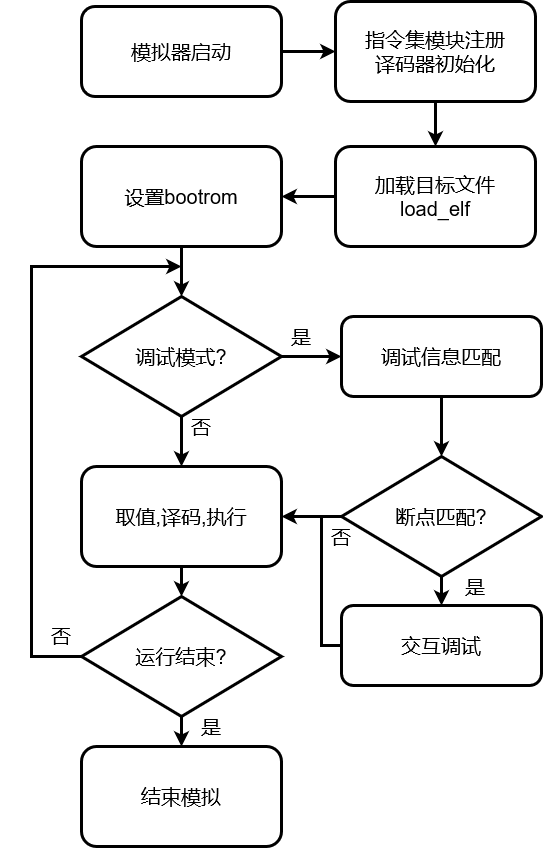
\includegraphics[width=0.5\textwidth]{sim-seq.png}
  \caption{模拟器运行流程图}
  \label{fig:sim-seq}
\end{figure}


首先使用RISC-V交叉编译工具链将目标程序编译为RISC-V架构的ELF文件,然后模拟器解析该elf文件,将对应的指令流搬运到bootrom,模拟器在配置启动后为处理器注册指令集,绑定解码器,逐条进行译码,执行。指令译码器完成包括操作数在内的指令信息提取,找到该条指令注册时对应的功能函数,执行该功能函数,然后将更新后的寄存器状态信息,内存状态信息同步到前端UI显示模块。在模拟器运行的过程中,用户还可以通过前端交互调试窗口来切换模拟器运行模式,设置断点触发条件,进行单步调试,状态查询等操作。

\subsection{解码器与指令集功能函数}
RISC-V指令集是模块化的,它的核心是一个名为RV32I的基础ISA,可选的标准扩展包括MAFDC,根据应用程序的需要,硬件可以包含或不包含这些扩展。本模拟器实现了特权指令集1.9版本,和用户指令集2.1版本的标准拓展指令集共196条指令的模拟。模拟器预加载时通过解析配置参数选择相应的指令集模块进行注册,并初始化解码器.流程如图~\ref{fig:decode-process}所示.
\begin{figure}[H]
  \centering
  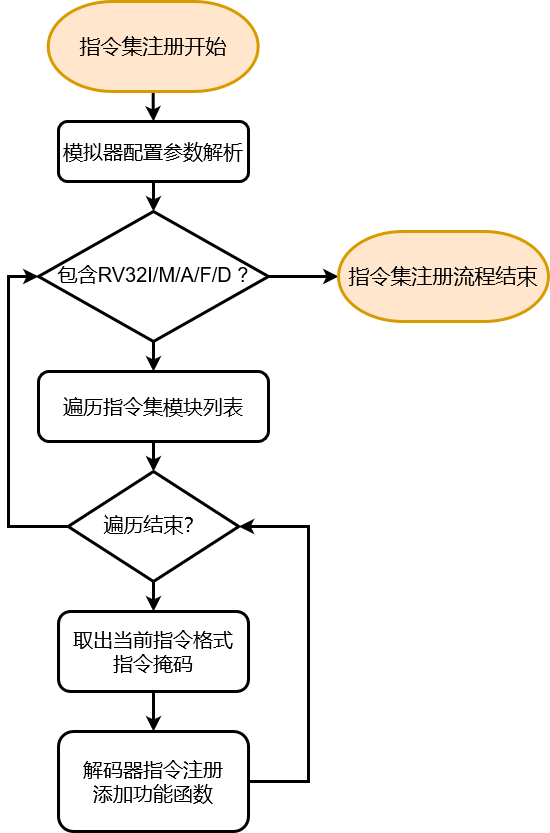
\includegraphics[width=0.5\textwidth]{decode-process.png}
  \caption{指令集模块注册流程图}
  \label{fig:decode-process}
\end{figure}


模拟器启动后首先根据配置参数解析需要加载的指令集模块,然后遍历各个模块的指令列表,将指令操作码格式和对应的功能函数注册到译码器当中,作为模拟目标机器的完备指令集,后续的目标函数执行过程均不超过当前注册的指令集范围,否则将会产生非法指令的异常导致模拟目标程序崩溃。

\subsection{指令流程控制}
在CPU运行过程中,存在两种指令流程,一种是常规的逻辑控制流,包括顺序的指令流和分支跳转;另一种称为异常控制流,用来响应处理器状态的某些变化,表现为中断或异常.之前的章节已将介绍了CPU指令控制流程的模拟,其中包括了响应中断的逻辑,CPU在取值之前检查当前是否有中断信号,根据状态寄存器判断是否响应中断,进入异常控制流逻辑.本节只讨论逻辑控制流的设计,异常控制流程设计将在下一节的中断控制中详细说明。


指令的执行,分为取指、译码、执行三个步骤。对于单条指令,在逻辑上这三个步骤是顺序的,同步的。所以对于功能模拟器,仍然可以把实际的流水线设计看作是单周期的CPU。处理器核的功能模拟主要包括存储管理单元MMU,高速缓存,以及寄存器组,这部分硬件功能模块都作为处理器核对象的私有成员;模拟器对象管理公有的内存部分,译码器,以及总线和外设.


MMU的功能模拟主要体现在处理器各个运行状态下的地址翻译功能.在真实的芯片设计中,缓存和MMU是两个独立的硬件模块,但是在功能模拟器中,为了实现的方便,可以将高速缓存模块放到MMU功能模块中,在逻辑上仍然属于两个独立的功能模块,这样做对于处理器行为的模拟没有影响.由于模拟器对于缓存的模拟只能记录缓存的命中率等信息,并不能够真正起到硬件加速的效果,此外本次设计的模拟器作为功能模拟器并不需要对处理器性能指标进行模拟,所以直接舍弃L2Cache的模拟,只在MMU模块中设置iCache和dCache,后续可以使用哈希的方式尝试进行部分优化.MMU和缓存的概要设计如图~\ref{fig:mmu-process}所示。
\begin{figure}[H]
  \centering
  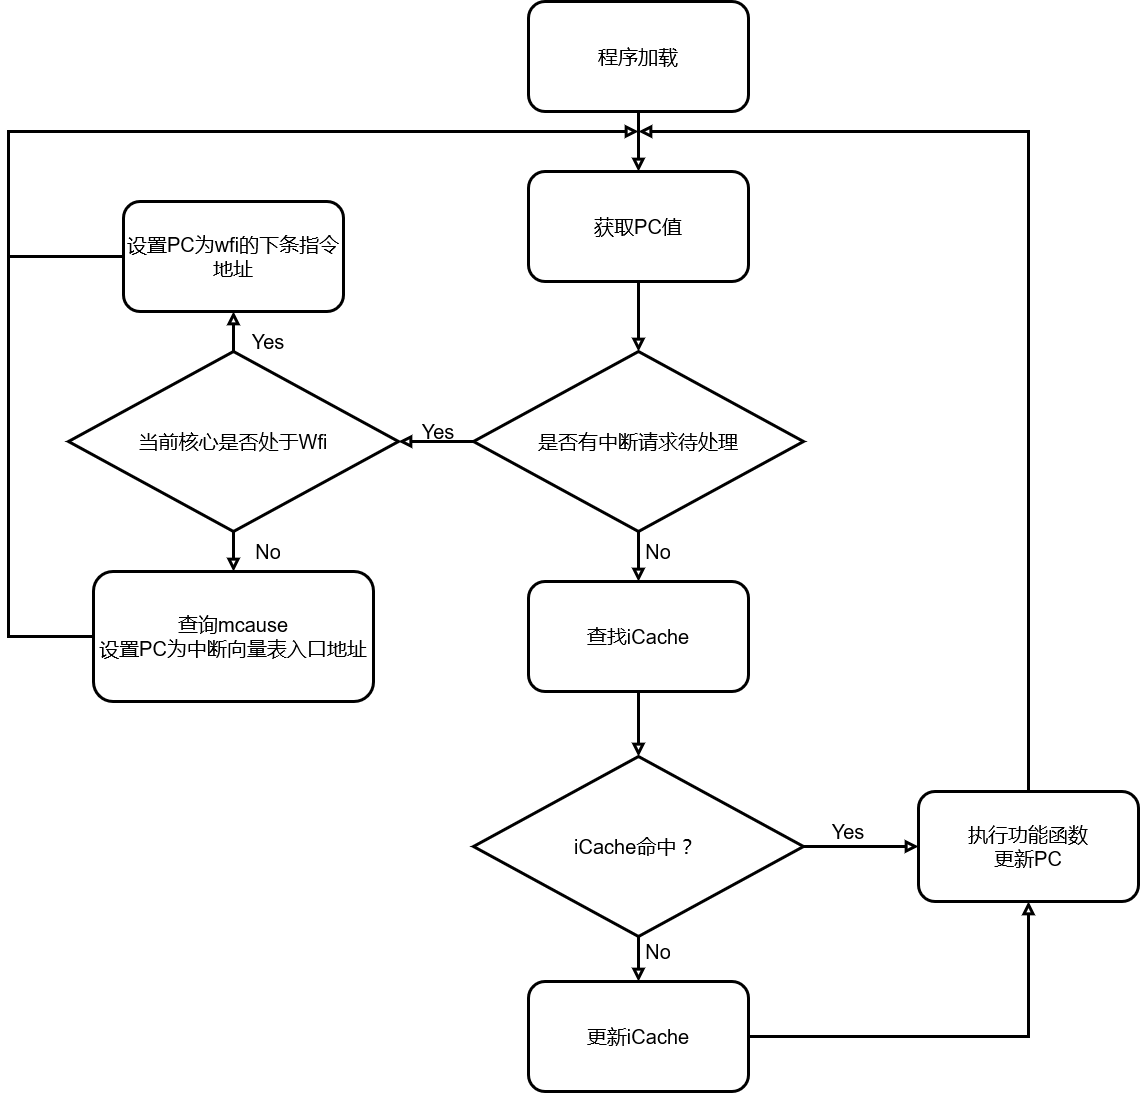
\includegraphics[width=0.95\textwidth]{mmu-process.png}
  \caption{MMU和缓存工作流程图}
  \label{fig:mmu-process}
\end{figure}


寄存器组的模拟需要参照汇编指令具体功能进行设计。单从数据层面上讲,寄存器组只是处理器内部的一组可随机存取的数据单元,实现上使用数组就可以模拟,但是对寄存器的操作是和汇编指令功能密切相关的,RISC-V指令级架构的设计充分发挥了后发优势,将寄存器id映射到指令操作码的固定位置,从硬件设计上来讲能够极大地简化电路设计,从软件模拟的角度讲,也更加方便于接口设计,使得后续的指令集功能函数实现能够逻辑清晰,实现起来代码逻辑也更加简洁。


对于总线的模拟,可以将其抽象成统一的通信中转信箱,由全局的模拟器对象维护,可以忽略实际总线的电气特性细节,对处理器核表现为统一的外设控制器,处理包括中断控制器,RTC,BootRom固件等的以内存映射方式寻址的外部设备的通信。

\subsection{中断控制器}
之前的章节已将介绍了CPU指令流程控制的设计,主要是取值/译码/执行的逻辑控制流程,本模拟器的一大设计需求就是要能够模拟器部分外设,从而进行对应驱动程序的开发和测试.大部分的外设都需要通过外部中断的方式与处理器核进行交互,所以本模拟器必须要实现平台级中断控制器PLIC,下面将介绍终端模块的整体设计.首先,对于中断模块的被动响应方,处理器核对于中断信号的响应需要在单个指令执行周期内完成,所以模拟器在单条汇编指令的取值动作之前将对处理器核的状态寄存器进行检查,判断当前是否有待处理的中断信号,然后完成相应的硬件动作;其次,对于中断的主动发起方,PLIC需要进行多个外部中断源的优先级裁决,控制中断源的使能情况,并对所有处理器核的优先级门限进行筛查,对符合条件的所有中断目标发起外部中断请求.PLIC连接到模拟器的所有处理器核心,对内表现为黑盒,处理器不关心中断控制器的内部逻辑,只针对相应的外部中断信号,以及中断源id,进行对应的中断响应.PLIC与处理器核的关系如图~\ref{fig:plic-to-hart}所示.
\begin{figure}[H]
  \centering
  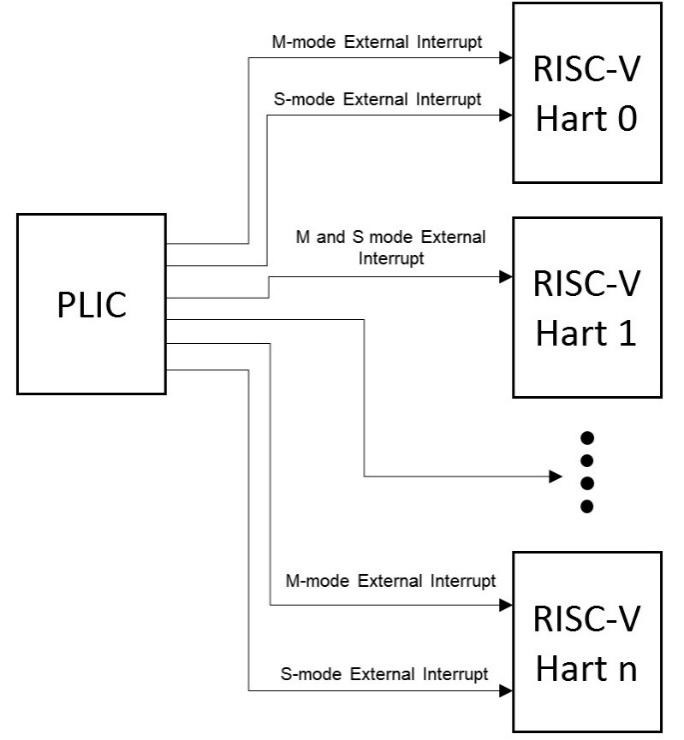
\includegraphics[width=0.7\textwidth]{plic-to-hart.jpg}
  \caption{PLIC外部中断}
  \label{fig:plic-to-hart}
\end{figure}
SiFive公司对PLIC整体架构做了规范,本模拟器按照该规范进行设计,具体的实现将在下一章介绍。该硬件模块对处理器核表现为黑盒,只提供固定功能的接口,整体作为外部设备通过总线与处理器进行通信。


\subsection{交互调试模块}
本模拟器的主要功能就是进行目标程序的调试工作,包括bootloader,linux内核,驱动程序等.因此本模拟器的设计不仅需要提供丰富的调试手段,还要能够提供友好的可视化界面,方便进行目标程序调试,加快系统软件的开发/测试/迭代周期.调试模块的功能集成在上述的处理器指令流程控制模块以及前端UI模块之中.其中,UI模块的可视化界面提供调试信息的设置,查询功能,后端模拟器指令执行流程中将对设置的调试信息进行匹配,将断点匹配结果,调试查询结果反馈到前端UI模块,与开发人员进行调试交互.该模块需要提供断点设置,单步执行,寄存器/内存查询等功能.UI显示界面主要包含了断点设置窗口,查询窗口和执行交互窗口.

\section{本章小结}
本章主要是根据系统的需求规格说明书,对RISC-V指令集模拟器进行概要设计,确定了本模拟器的四个主要功能模块:指令集模块,CPU和总线模块,中断模块,以及交互调试模块.描述了模拟器整体运行流程,并对各模块的功能逻辑进行设计,明确了RISC-V指令集模拟器的总体框架,动态流程以及各模块设计方案.